\section{Deep unsupervised learning}\label{sec:unsup}
%Previous two sections are devoted to supervised learning, where one is given a labeled dataset $\{(\bm{x}_{i},y_{i})\}_{1\leq i\leq n}$ and wish to learn a mapping from the input $\bm{x}$ to the label $y$.


In supervised learning, given labelled training set $\{(y_i,\bx_i)\}$, we focus on discriminative models, which essentially represents $\P(y\,|\,\xx)$ by a deep neural net $f(\xx; \btheta)$ with parameters $\btheta$. Unsupervised learning, in contrast, aims at extracting \emph{information} from \emph{unlabeled} data $\{\bm{x}_{i}\}$, where the labels $\{y_i\}$ are absent. In regard to this information, it can be a low-dimensional embedding of the data $\{ \xx_i \}$ or a generative model with latent variables to approximate the distribution $\P_{\bX}(\xx)$. To achieve these goals, we introduce two popular unsupervised deep leaning models, namely, autoencoders and generative
adversarial networks~(GANs). The first one can be viewed as a dimension reduction technique, and the second as a density estimation method. DNNs are the key elements for both of these two models. %To this end, here we will need two deep neural nets to represent maps between $\xx$ and its low-dimensional representation $\zz$: encoder/decoder in autoencoders, and discriminator/generator in GANs.


\subsection{Autoencoders}
Recall that in dimension reduction, the goal is to reduce the dimensionality of the data and at the same time preserve its salient features. In particular, in principal component analysis (PCA), the goal is to embed the data $\{\bm{x}_{i}\}_{1\leq i\leq n}$ into a low-dimensional space via a linear function $\ff$ such that maximum variance can be explained. Equivalently, we want to find linear functions $\ff: \R^d \to \R^k$ and $\bgg: \R^k \to \R^d$ ($k \le d$) such that the difference between $\xx_i$ and $\bgg(\ff(\xx_i))$ is minimized. Formally, we let
\[
\ff\left(\bm{x}\right)=\bm{W}_f\bm{x}\triangleq \hh \quad\text{and}\quad \bgg\left(\bm{h}\right)=\bm{W}_g\bm{h}, \quad \text{where}\quad\bm{W}_f\in\mathbb{R}^{k\times d}\text{ and } \bm{W}_g\in\mathbb{R}^{d\times k}.
\]
Here, for simplicity, we assume that the intercept/bias terms for $\ff$ and $\bgg$ are zero. Then, PCA amounts to minimizing the quadratic loss function
\begin{equation}
\text{minimize}_{\bm{W}_f, \bm{W}_g}\qquad \frac{1}{n} \sum_{i=1}^{n}\left\Vert \bm{x}_i-\bm{W}_f\bm{W}_g\bm{x}_i\right\Vert _{2}^{2}.\label{eq:linear-AE}
\end{equation}
It is the same as minimizing $\| \bX - \bW \bX \|_{\mathrm{F}}^2$ subject to $\rank(\bW) \le k$, where $\bX\in \mathbb{R}^{p\times n}$ is the design matrix. The solution is given by the singular value decomposition of $\bX$ \citep[Thm.~2.4.8]{golub2013matrix}, which is exactly what PCA does. It turns out that PCA is a special case of autoencoders, which is often known as the \textit{undercomplete linear autoencoder}.

More broadly, autoencoders are neural network models for (nonlinear) dimension reduction, which generalize PCA. An autoencoder has two key components, namely, the encoder function $\ff(\cdot)$, which maps the input $\bm{x}\in\mathbb{R}^{d}$ to a hidden code/representation $\bm{h}\triangleq\ff(\bm{x})\in\mathbb{R}^{k}$, and the decoder function $\bgg(\cdot)$, which maps the hidden representation $\bm{h}$ to a point $\bgg(\bm{h})\in\mathbb{R}^{d}$. Both functions can be multilayer neural networks as \eqref{eq:fc}. See Figure~\ref{fig:AE} for an illustration of autoencoders. Let $\mathcal{L}(\bm{x}_{1},\bm{x}_{2})$ be a loss function that measures the difference between $\bm{x}_{1}$ and $\bm{x}_{2}$ in $\R^d$. Similar to PCA, an autoencoder is used to find the encoder $\ff$ and decoder $\bgg$ such that $\mathcal{L}(\bm{x},\bgg(\ff(\bm{x})))$
is as small as possible. Mathematically, this amounts to solving the following minimization problem
\begin{equation}
\mbox{minimize}_{\ff,\bgg} \quad\frac{1}{n}\sum_{i=1}^{n}\mathcal{L}\left(\bm{x}_{i},\bgg\left(\bm{h}_{i}\right)\right) \quad \text{with}\quad\bm{h}_{i}=\ff\left(\bm{x}_{i}\right), \quad \text{for all }\, i \in [n].  \label{eq:AE}
\end{equation}
\begin{figure}
\centering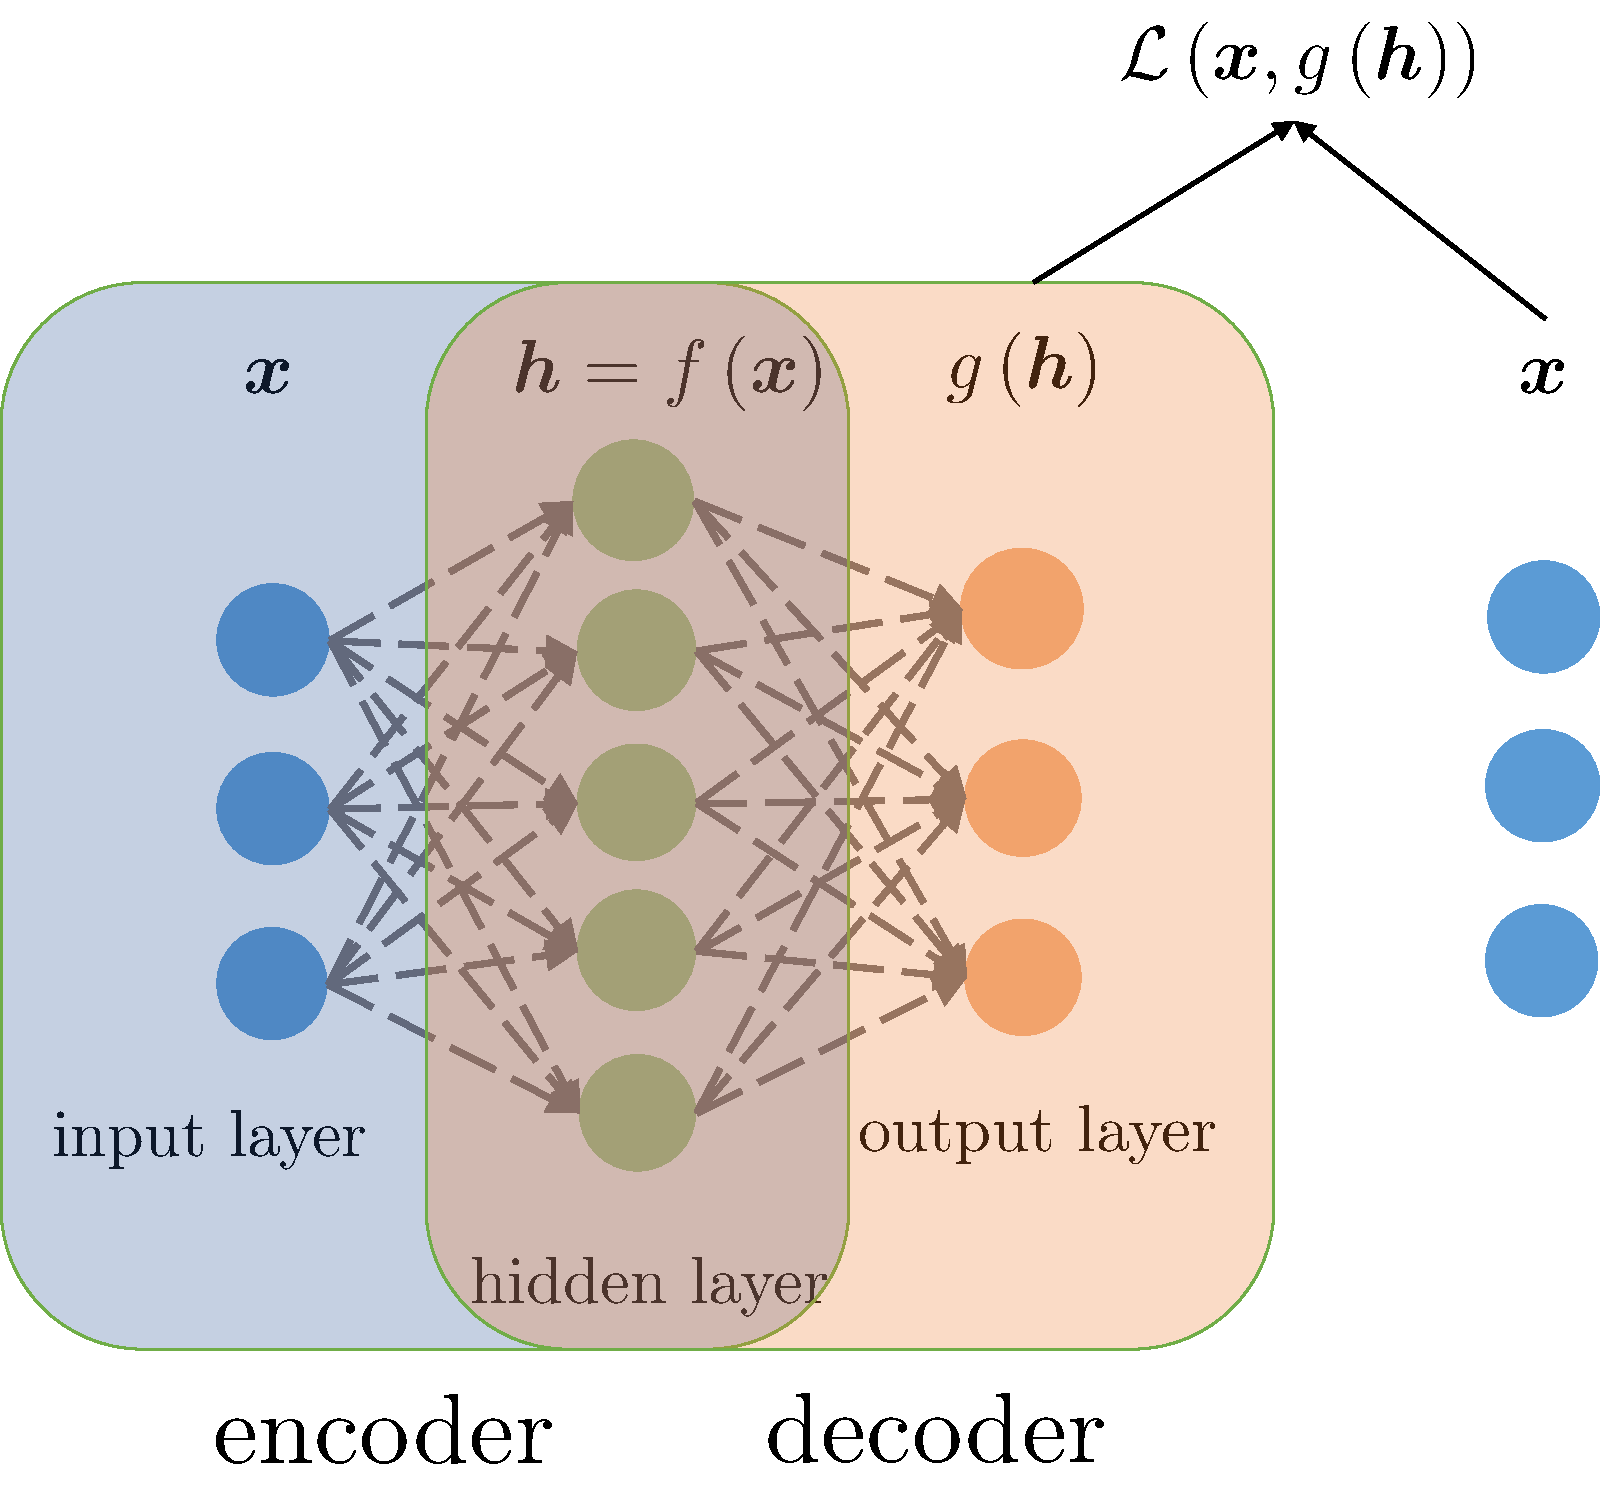
\includegraphics[scale=0.3]{AE}
\caption{First an input $\bm{x}$ goes through the decoder $\ff(\cdot)$, and we obtain its hidden representation $\bm{h}= \ff(\bm{x})$. Then, we use the decoder $\bgg(\cdot)$ to get $\bgg(\bm{h})$ as a reconstruction of $\bm{x}$. Finally, the loss is determined from the difference between the original input $\bm{x}$ and its reconstruction $\bgg(\ff(\bm{x}))$.}\label{fig:AE} %\TODO{give more than one layer}
\end{figure}

One needs to make structural assumptions on the functions $\ff$ and $\bg$ in order to find useful representations of the data, which leads to different types of autoencoders. Indeed, if no assumption is made, choosing $\ff$ and $\bgg$ to be identity functions clearly minimizes the above optimization problem. To avoid this trivial solution, one natural way is to require that the encoder $f$ maps the data onto a space with a smaller dimension, i.e., $k < d$. This is the \textit{undercomplete autoencoder} that includes PCA as a special case. There are other structured autoencoders which add desired properties to the model such as sparsity or robustness, mainly through regularization terms. Below we present two other common types of autoencoders.

\begin{itemize}
\item \emph{Sparse autoencoders. } One may believe that the dimension $k$ of the hidden code $\hh_i$ is larger than the input dimension $d$, and that $\hh_i$ admits a sparse representation. As with LASSO \citep{tibshirani1996regression} or SCAD \citep{fan2001variable}, one may add a regularization term to the reconstruction loss $\mathcal{L}$ in \eqref{eq:AE} to encourage sparsity \citep{poultney2007efficient}. A sparse autoencoder solves
\begin{equation*}
\mbox{min}_{\ff,\bgg}  \; \underbrace{ \frac{1}{n}\sum_{i=1}^{n}\mathcal{L}\left(\bm{x}_{i},\bgg\left(\bm{h}_{i}\right)\right) }_{\text{loss}}+ \underbrace{\vphantom{\frac{1}{n}\sum_{i=1}^{n}\mathcal{L}\left(\bm{x}_{i},\bgg\left(\bm{h}_{i}\right)\right)} \lambda\left\Vert \bm{h}_{i}\right\Vert _{1} }_{\text{regularizer}} \quad \text{with} \quad \bm{h}_{i}=\ff\left(\bm{x}_{i}\right), \text{ for all } i \in [n].
\end{equation*}
This is similar to \textit{dictionary learning}, where one aims at finding a sparse representation of input data on an overcomplete basis. Due to the imposed sparsity, the model can potentially learn useful features of the data.

\item \emph{Denoising autoencoders. } One may hope that the model is robust to noise in the data: even if the input data $\bm{x}_i$ are corrupted by small noise $\bxi_i$ or miss some components (the noise level or the missing probability is typically small), an ideal autoencoder should faithfully recover the original data. A denoising autoencoder \citep{vincent2008extracting} achieves this robustness by explicitly building a noisy data $\tilde{\bm{x}}_{i} = \bm{x}_i + \bxi_i$ as the new input, and then solves an optimization problem similar to \eqref{eq:AE} where $\mathcal{L}\left(\bm{x}_{i},\bgg\left(\bm{h}_{i}\right)\right)$ is replaced by $\mathcal{L}\left(\bm{x}_{i},\bgg\left(\ff(\tilde{\bm{x}}_{i})\right)\right)$. A denoising autoencoder encourages the encoder/decoder to be stable in the neighborhood of an input, which is generally a good statistical property. An alternative way could be constraining $f$ and $g$ in the optimization problem, but that would be very difficult to optimize. Instead, sampling by adding small perturbations in the input provides a simple implementation. We shall see similar ideas in Section~\ref{sec:aug}.
    %{\bf Q: where is the regularization: noisy + unnoisy data?}

%\item \emph{Variational autoencoders. } Just as PCA has a probabilistic (or generative) underpinning, namely factor models, autoencoders \eqref{eq:AE} can also be cast in the language of latent variable models. Let the latent variables $\hh$ be $\mathcal{N}(\bzero, \bI_k)$, and suppose the conditional probability $p_{\btheta}(\xx | \hh)$ is associated with a decoder neural network with parameters $\btheta$; for example, $\xx = \bg_{\btheta}(\hh) + \sigma \cdot \mathcal{N}(\bzero, \bI_d)$. To find the MLE for $\btheta$, one difficulty is to compute $p_{\btheta}(\xx)$, which involves complicated integral after expanding this probability in term of $\hh$. The idea of variational autoencoders is to use an encoder neural network $f_{\bvarphi}$ to approximate the posterior $p_{\btheta}(\hh | \xx)$. See \cite{doersch2016tutorial} for details of derivation and examples. Similar to the aforementioned autoencoders, the final optimization formulation of variational autoencoders involves a loss term that represents the reconstruction error, and a Kullback-Leibler divergence that serves as a regularizer.

\end{itemize}

\subsection{Generative adversarial networks}

Given unlabeled data $\{\bm{x}_{i}\}_{1\leq i\leq n}$, density estimation
aims to estimate the underlying probability density function $\mathbb{P}_{\bm{X}}$
from which the data is generated. Both parametric and nonparametric
estimators \citep{silverman2018density} have been proposed and studied under various assumptions
on the underlying distribution. Different from these classical density estimators, where the density function is explicitly defined in relatively low dimension, generative adversarial networks (GANs) \citep{goodfellow2014generative} can be categorized as an \emph{implicit} density estimator in much higher dimension. The reasons are twofold: (1) GANs put more emphasis on sampling from
the distribution $\mathbb{P}_{\bm{X}}$ than estimation; (2) GANs define the density estimation implicitly through a source distribution $\mathbb{P}_{\bm{Z}}$ and a generator function $g(\cdot)$, which is usually a deep neural network. We introduce GANs from the perspective of sampling from $\mathbb{P}_{\bm{X}}$ and later we will generalize the vanilla GANs using its relation to density estimators.

\subsubsection{Sampling view of GANs}
Suppose the data $\{\bm{x}_{i}\}_{1\leq i\leq n}$ at hand are all real images, and we want to generate \emph{new} natural images.
With this goal in mind, GAN models a \emph{zero-sum} game between two players, namely,
the generator $\mathcal{G}$ and the discriminator $\mathcal{D}$. The
generator $\mathcal{G}$ tries to generate fake images akin to the
true images $\{\bm{x}_{i}\}_{1\leq i\leq n}$ while the discriminator
$\mathcal{D}$ aims at differentiating the fake ones from
the true ones. Intuitively, one hopes to learn a generator $\mathcal{G}$ to generate images where the \emph{best} discriminator $\mathcal{D}$ cannot distinguish. Therefore the payoff is higher for the generator~$\mathcal{G}$ if the probability of the discriminator $\mathcal{D}$
getting wrong is higher, and correspondingly the payoff for the discriminator
correlates positively with its ability to tell wrong from truth.

Mathematically, the generator $\mathcal{G}$ consists of two components,
an source distribution $\mathbb{P}_{\bm{Z}}$ (usually a standard multivariate Gaussian distribution with hundreds of dimensions) and a function $\bg(\cdot)$ which maps a sample
$\bm{z}$ from $\mathbb{P}_{\bm{Z}}$ to a point $\bg(\bm{z})$ living
in the same space as $\bm{x}$. For generating images, $\bg(\bm{z})$ would be a 3D tensor. Here $\bg(\bm{z})$ is the fake sample
generated from $\mathcal{G}$. Similarly the discriminator $\mathcal{D}$
is composed of one function which takes an image ${\bm{x}}$ (real or fake)
and return a number $d({\bm{x}})\in[0,1]$, the probability
of ${\bm{x}}$ being a real sample from $\mathbb{P}_{\bm{X}}$ or not.
Oftentimes, both the generating function $\bg(\cdot)$ and the discriminating
function $d(\cdot)$ are realized by deep neural networks, e.g., CNNs introduced in Section~\ref{sec:CNN}. See Figure~\ref{fig:GAN} for an illustration
for GANs. Denote $\btheta_{\mathcal{G}}$ and $\btheta_{\mathcal{D}}$
the parameters in $\bg(\cdot)$ and $d(\cdot)$, respectively. Then
GAN tries to solve the following \emph{min-max }problem:
\begin{figure}
\centering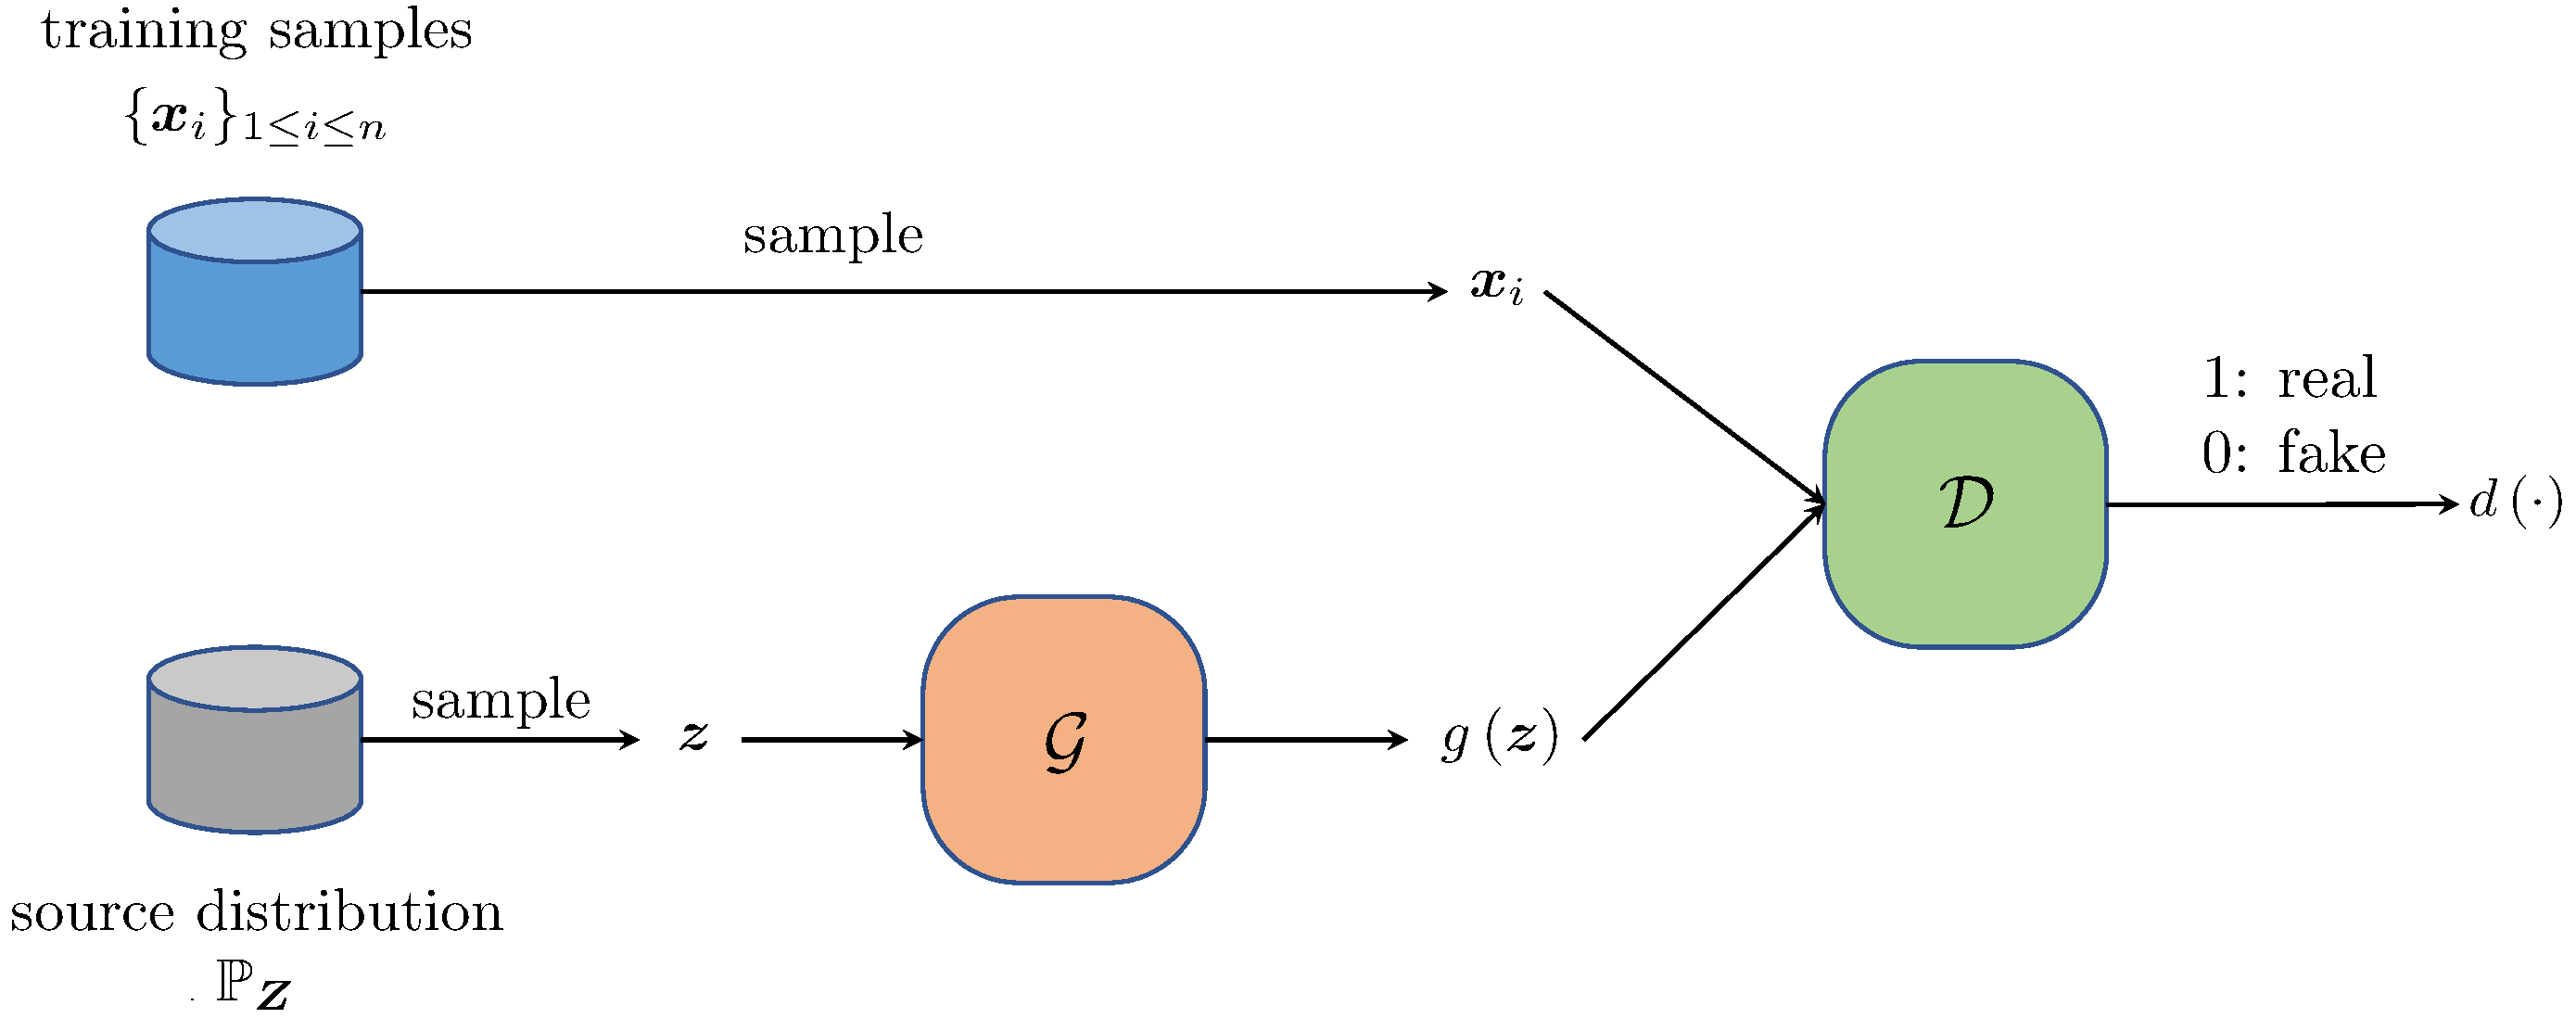
\includegraphics[width=0.9\textwidth]{GAN}
\caption{GANs consist of two components, a generator $\mathcal{G}$ which generates fake samples and a discriminator $\mathcal{D}$ which differentiate the true ones from the fake ones. \label{fig:GAN}}
\end{figure}
\begin{equation}
\min_{\btheta_{\mathcal{G}}}\max_{\btheta_{\mathcal{D}}}
\qquad\mathbb{E}_{\bm{x}\sim\mathbb{P}_{\bm{X}}}\left[\log
\left(d\left(\bm{x}\right)\right)\right]
+\mathbb{E}_{\bm{z}\sim\mathbb{P}_{\bm{Z}}}\left[\log\left(1-d\left(\bg\left(\bm{z}\right)\right)\right)\right].\label{eq:GAN-original}
\end{equation}
Recall that $d(\bm{x})$ models the belief / probability that the
discriminator thinks that $\bm{x}$ is a true sample. Fix the parameters
$\btheta_{\mathcal{G}}$ and hence the generator $\mathcal{G}$ and
consider the inner maximization problem.
We can see that the goal
of the discriminator is to maximize its ability of differentiation.
Similarly, if we fix $\btheta_{\mathcal{D}}$ (and hence the discriminator),
the generator tries to generate more realistic images $\bg(\bm{z})$
to fool the discriminator.

\subsubsection{Density estimation view of GANs}
Let us now take a density-estimation view of GANs. Fixing the source distribution $\mathbb{P}_{\bm{Z}}$, any generator $\mathcal{G}$ induces a distribution $\mathbb{P}_{\mathcal{G}}$ over the space of images. Removing the restrictions on $d(\cdot)$, one can then rewrite (\ref{eq:GAN-original}) as
\begin{equation}\label{eq:GAN-new}
\min_{\mathbb{P}_{\mathcal{G}}}\max_{d(\cdot)}\qquad\mathbb{E}_{\bm{x}\sim\mathbb{P}_{\bm{X}}}\left[\log\left(d\left(\bm{x}\right)\right)\right]+\mathbb{E}_{\bm{x}\sim\mathbb{P}_{\mathcal{G}}}\left[\log\left(1-d\left(\bm{x}\right)\right)\right].
\end{equation}
Observe that the inner maximization problem
is solved by the likelihood ratio,~i.e.
\[
d^{*}\left(\bm{x}\right)=\frac{\mathbb{P}_{\bm{X}}\left(\bm{x}\right)}{\mathbb{P}_{\bm{X}}\left(\bm{x}\right)+\mathbb{P}_{\mathcal{G}}\left(\bm{x}\right)}.
\]
As a result, (\ref{eq:GAN-new}) can be simplified as
\begin{equation}
\min_{\mathbb{P}_{\mathcal{G}}}\qquad\text{JS}\left(\mathbb{P}_{\bm{X}}\;\|\;\mathbb{P}_{\mathcal{G}}\right)\label{eq:JS-min},
\end{equation}
where $\text{JS}(\cdot\|\cdot)$ denotes the Jensen--Shannon divergence
between two distributions
\[
\text{JS}\left(\mathbb{P}_{\bm{X}}\|\mathbb{P}_{\mathcal{G}}\right)=\frac{1}{2}\text{KL}\big(\mathbb{P}_{\bm{X}}\;\|\;\tfrac{\mathbb{P}_{\bm{X}}+\mathbb{P}_{\mathcal{G}}}{2}\big)+\frac{1}{2}\text{KL}\big(\mathbb{P}_{\mathcal{G}}\;\|\;\tfrac{\mathbb{P}_{\bm{X}}+\mathbb{P}_{\mathcal{G}}}{2}\big).
\]
In words, the vanilla GAN (\ref{eq:GAN-original}) seeks a density $\mathbb{P}_{\mathcal{G}}$ that is closest to $\mathbb{P}_{\bm{X}}$ in terms of the Jensen--Shannon divergence. This view allows to generalize GANs to other variants, by changing the distance metric. Examples include f-GAN \citep{nowozin2016f}, Wasserstein GAN (W-GAN) \citep{arjovsky2017wasserstein}, MMD GAN \citep{li2015generative}, etc. We single out the Wasserstein GAN (W-GAN) \citep{arjovsky2017wasserstein} to introduce due to its popularity. As the name suggests, it minimizes
the Wasserstein distance between $\mathbb{P}_{\bm{X}}$ and $\mathbb{P}_{\mathcal{G}}$:
\begin{equation}
\min_{\btheta_{\mathcal{G}}}\quad \text{WS}\left(\mathbb{P}_{\bm{X}}\|\mathbb{P}_{\mathcal{G}}\right)\;\;=\;\;\min_{\btheta_{\mathcal{G}}}\sup_{f:f\text{ 1-Lipschitz}}\mathbb{E}_{\bm{x}\sim\mathbb{P}_{\bm{X}}}
\left[f\left(\bm{x}\right)\right]-\mathbb{E}_{\bm{x}\sim
\mathbb{P}_{\mathcal{G}}}\left[f\left(\bm{x}\right)\right],\label{eq:WS-GAN}
\end{equation}
where $f(\cdot)$ is taken over all Lipschitz functions with coefficient 1.
Comparing W-GAN (\ref{eq:WS-GAN}) with the original formulation of GAN (\ref{eq:GAN-original}), one finds
that the Lipschitz function $f$ in (\ref{eq:WS-GAN}) corresponds
to the discriminator $\mathcal{D}$ in (\ref{eq:GAN-original}) in the sense that they
share similar objectives to differentiate the true distribution
$\mathbb{P}_{\bm{X}}$ from the fake one $\mathbb{P}_{\mathcal{G}}$. In the end, we would like to mention that GANs are more difficult to train than supervised deep learning models such as CNNs~\citep{salimans2016improved}. Apart from the training difficulty, how to evaluate GANs objectively and effectively is an ongoing research.


%%%%%%%%%%%%%%%%
%%%%%%%%%%%%%%%%
\begin{comment}
\subsection{Note}
There are other types of autoencoders. In a contractive autoencoder \citep{rifai2011contractive}, one regularizes the encoder $f(\cdot)$ with a penalty on the gradients of the mapping so as to encourage smoothness. The autoencoders introduced herein can also be stacked together to form deep autoencoders \citep{hinton2006reducing, vincent2010stacked}. Stacked autoencoders was originally used as a pre-training technique to train deep neural networks \citep{hinton2006reducing}. %\TODO{stacked autoencoder is a model, not training technique? mention Boltzmann machine?}
Specifically, we can train the autoencoders layer by layer using only unlabeled data, after which we can discard the decoder component and view the encoders as feed-forward connections in usual neural networks. Connecting the top-layer with a classification layer, we can then fine-tune the parameters (that is, using parameters of the encoder as initial values) using the labels by back-propagation. However, its role in training deep neural nets is diminishing, and recent years have witnessed a trend where deep neural nets are directly trained without resorting to autoencoders as pre-training.

%Many other generative models, such as the restricted Boltzmann machine, predated the popularity of deep neural nets. \TODO{some intro here; due to its historical imporantance.}

GANs, popular for their surprising ability to generate real images, are also notorious for their training difficulty \citep{goodfellow2016nips,radford2015unsupervised,salimans2016improved}. It is still an active research area to develop better network architectures and training algorithms for GANs.
\end{comment}

%%%%%%%%%%%%%%%%
%%%%%%%%%%%%%%%% 